%%%%%%%%%%%%%%%%%%%%%%%%%%%%%%%%%%%%%%%%%%%%%%%%%%%%%%%%%%%%%%%%%%%%%%%%%%%%%%%%%%
%%%%%  								LuaLatex								 %%%%%
%%%%%%%%%%%%%%%%%%%%%%%%%%%%%%%%%%%%%%%%%%%%%%%%%%%%%%%%%%%%%%%%%%%%%%%%%%%%%%%%%%
\documentclass[11pt,aspectratio=43,mathserif]{beamer}
\usetheme[numbering=none, progressbar=none, sectionpage=none , block=fill]{metropolis} %numbering=fraction,

\setsansfont{Arial}      % set main font
%\setsansfont{Myriad Pro}
\usepackage[style=ieee,sorting=nyt]{biblatex}
\addbibresource{biblio.bib}
\usepackage{color}
\setmonofont{Consolas}
\usepackage{arevmath}
\usepackage{appendixnumberbeamer}
\usepackage{booktabs}
\usepackage[scale=2]{ccicons}
\usepackage{media9}
\usepackage{pgfplots}
\graphicspath{{./figures/}}
\addmediapath{{./movies/}}
\pgfplotsset{compat=newest}
\pgfplotsset{plot coordinates/math parser=false} 
\newlength\figurewidth
\newlength\figureheight

\definecolor{TueRed}{HTML}{cf0545}
%\definecolor{TueText}{HTML}{003A80}
\definecolor{TueBlue}{HTML}{00a6d6}
\definecolor{TueWarm}{HTML}{f54029}
\definecolor{TueText}{RGB}{0,58,128}

\definecolor{PMS206}{HTML}{d6004a}
\definecolor{PMSWarmRed}{HTML}{f73131}
\definecolor{PMS226}{HTML}{d6007b}
\definecolor{PMS253}{HTML}{ad20ad}
\definecolor{PMS2748}{HTML}{101073}
\definecolor{PMS300}{HTML}{0066cc} 
\definecolor{PMSProcessCyan}{HTML}{00a2de}
\definecolor{PMS137}{HTML}{ff9a00}

\setbeamercolor{frametitle}{fg=white, bg=TueRed}
\setbeamercolor{progress bar}{fg=TueRed}
\setbeamercolor{normal text}{fg=TueText, bg=white}
\setbeamercolor{title}{fg=TueText, bg=white}
\setbeamercolor{background canvas}{fg=black, bg=white}
\setbeamercolor{math text}{fg=TueText, bg=white}
\setbeamercolor{math text displayed}{fg=TueText, bg=white}

\definecolor{Block}{HTML}{ededed}
\setbeamercolor{block title}{bg=TueRed,fg=white}
\setbeamercolor{block body}{bg=Block,fg=TueText}
%\setbeamercolor{block title}{bg=TueText,fg=white}
%\setbeamercolor{block body}{bg=TueBlue,fg=white}
%\setbeamerfont{frametitle}{size=\Large}
\setbeamerfont{institute}{size=\footnotesize}

\setbeamertemplate{bibliography item}[text]
\usepackage{mhchem}
\usepackage[per-mode=symbol]{siunitx}
\AtBeginDocument{\sisetup{math-rm=\mathrm, text-rm=\rmfamily}} %\si 

\usepackage{amsmath}
\usepackage{mathspec}
\setmathfont(Digits){Arial}

\usepackage{caption}

\DeclareCaptionLabelFormat{mycaption}{\usebeamercolor[fg]{caption name}#1#2 \,\,}
\captionsetup[figure]{labelformat=mycaption, labelsep=none, labelfont=sf} %sc
\captionsetup[table]{labelformat=mycaption, labelsep=none, labelfont=sf} %sc
\setbeamerfont{caption}{series=\normalfont,size=\footnotesize}

\renewcommand{\figurename}{Fig.\,}
\renewcommand{\tablename}{Tab.\,}
%%%%%%%%%%%%%%%%%%%%%%%%%%%%%%%%%%%%%%%%%%%%%%%%%%%%%%%%%%%%%%%%%%%%%%%%%%%%%%%%%
%%%%%								COMMANDS								%%%%%
%%%%%%%%%%%%%%%%%%%%%%%%%%%%%%%%%%%%%%%%%%%%%%%%%%%%%%%%%%%%%%%%%%%%%%%%%%%%%%%%%

\newcommand{\includemovie}[1]{%
\includemedia[%
	width=\textwidth , height=0.55\textwidth,
	activate=pagevisible,%
	deactivate=pageclose,%
	addresource=#1,%
	flashvars={%
		src=#1 % same path as in addresource!
		&autoPlay=true %
		&loop=false % 
		&scaleMode=letterbox
		&autoRewind=false
		&muted=true
		&controlBarAutoHideTimeout=0 %  time span before auto-hide
		%&deactivate=onclick %faster
}%
]{}{StrobeMediaPlayback.swf}}%



\begin{document}
\nocite{*} %% All sources

\title{Optimization of the Heating Process for Offshore Wind Turbine Foundations}
\author{T.M.J. Bouts}
\institute{\today \\
Eindhoven University of Technology}
\titlegraphic{%
  \makebox[\textwidth]{%
    
\includegraphics[height=0.95cm]{Tue_logo2.pdf}%
    \hfill%
    
\includegraphics[height=0.95cm]{Microsystems_logo.pdf}%
    \hspace*{0.5cm}
  }%
}
\makeatletter
\setbeamertemplate{title page}{
  \vspace*{-30mm}\begin{minipage}[b][\paperheight]{\textwidth}
    \centering
    \ifx\inserttitle\@empty\else\usebeamertemplate*{title}\fi
    \ifx\insertsubtitle\@empty\else\usebeamertemplate*{subtitle}\fi
    \usebeamertemplate*{title separator}
    \ifx\beamer@shortauthor\@empty\else\usebeamertemplate*{author}\fi
    %\vspace*{5mm}
    \ifx\insertinstitute\@empty\else\usebeamertemplate*{institute}\fi
	%\vspace*{-5mm}
    \ifx\inserttitlegraphic\@empty\else\usebeamertemplate*{title graphic}\fi
  \end{minipage}
}

\setbeamertemplate{title}{
  \linespread{1.0}%
  {\Large\inserttitle}%
  \par%
  \vspace*{0.5em}
}
\setbeamertemplate{subtitle}{
  \insertsubtitle%
  \par%
  \vspace*{0.5em}
}

\makeatother
\begin{frame}[noframenumbering]
    \titlepage
    \thispagestyle{empty}
\end{frame}

%\begingroup
%\large

\begin{frame}{Contents}
\tableofcontents[hideallsubsections]
\end{frame}
\section{Introduction}

\begin{frame}{Introduction}
  \begin{columns}[onlytextwidth]
    \column{0.5\textwidth}
      \begin{itemize}
        \item 80m monopole
        \begin{itemize}
       		\item[--] Piles welded together
	    \end{itemize}    
	    \pause    
        \item Minimum 100 $^{\circ} \text{C}$
        \pause
        \item Propane \& Natural gas
      \end{itemize}

    \column{0.5\textwidth}
		\begin{figure}[H]
			\hfill 
			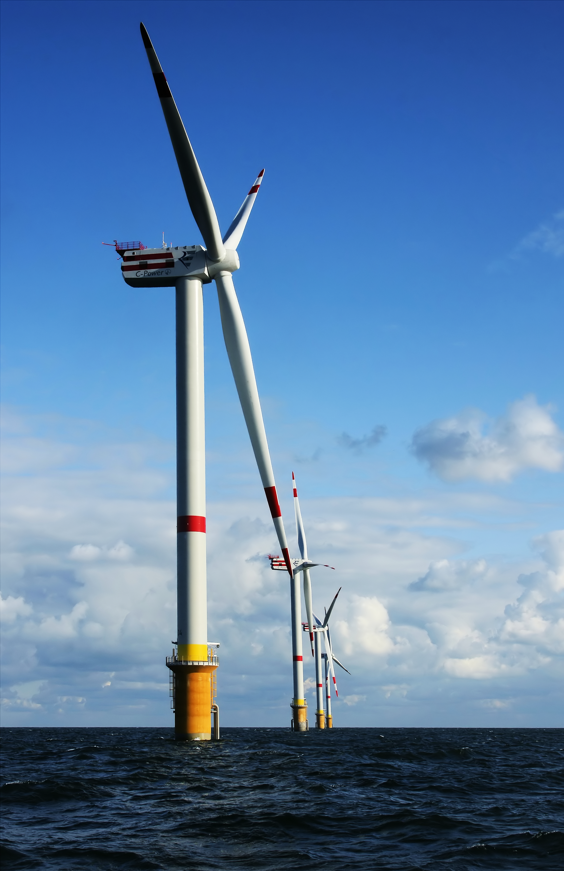
\includegraphics[width=.9\linewidth]{figures/Windmill.png}
			%\caption{}
			%\label{fig:}
		\end{figure} 
  \end{columns}
\end{frame}

\begin{frame}
	$1 2 3 4 5 6 7 8 9 0$ math \\
	1234567890 no math
\end{frame}

\begin{frame}{Introduction}
	\begin{itemize}
		\item Cost reduction by changing burner configuration
		\item Burner to pile
		\begin{itemize}
			\item[--] Burner types
			\item[--] Different fuels
			\item[--] Heat flux as a function of position
		\end{itemize}				
		\item Heat transfer in the pile
\end{itemize}
\end{frame}

\begin{frame}{Adiabatic flame temperature}
	\begin{figure}[H]
		\centering 
		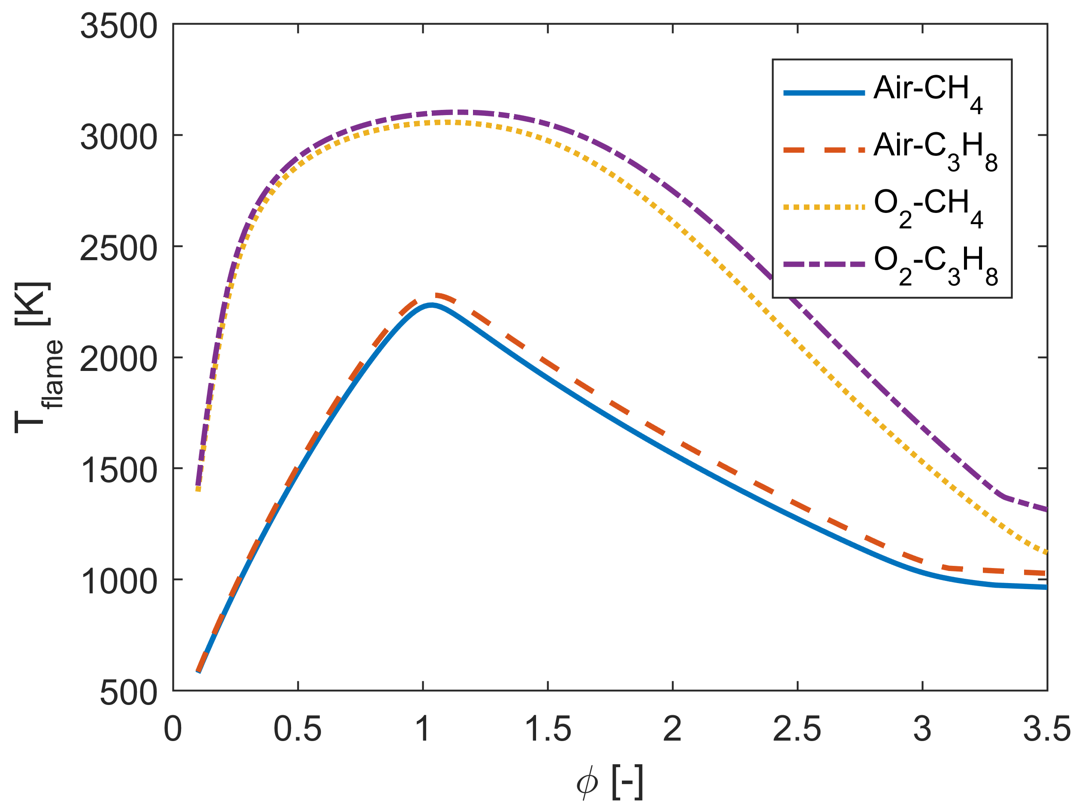
\includegraphics[width=0.8\linewidth]{ad.png}
		%\caption{A figure with flames}
	\end{figure} 
\end{frame}

\begin{frame}{Tikz Figure}
\vspace*{-2mm}
	\begin{figure}
		\setlength\figurewidth{0.8\textwidth}
		\setlength\figureheight{0.6\textwidth}
		\centering		
		% This file was created by matlab2tikz.
%
\definecolor{mycolor1}{rgb}{0.00000,0.44700,0.74100}%
\definecolor{mycolor2}{rgb}{0.85000,0.32500,0.09800}%
\definecolor{mycolor3}{rgb}{0.92900,0.69400,0.12500}%
\definecolor{mycolor4}{rgb}{0.49400,0.18400,0.55600}%
%
\begin{tikzpicture}

\begin{axis}[%
width=0.951\figurewidth,
height=\figureheight,
at={(0\figurewidth,0\figureheight)},
scale only axis,
xmin=0,
xmax=3.5,
xlabel style={font=\color{white!15!black}},
xlabel={$\phi$ [\si{-}]},
ymin=500,
ymax=3500,
ylabel style={font=\color{white!15!black}},
ylabel={$T_{\textsf{flame}}$ [\si{K}]},
axis background/.style={fill=white},
legend style={legend cell align=left, align=left, draw=white!15!black},
xlabel style={font=\footnotesize},ylabel style={font=\footnotesize},y tick label style={/pgf/number format/.cd,scaled y ticks = false, set thousands separator={},fixed},legend style={font=\sffamily\footnotesize,draw=TueText},ticklabel style={font=\sffamily\footnotesize}
]
\addplot [color=mycolor1, line width=1.5pt]
  table[row sep=crcr]{%
0.0999999999999091	578.93564750138\\
0.151256281406859	712.778495026967\\
0.202512562814263	840.109027687692\\
0.253768844221213	961.371219596829\\
0.322110552763661	1115.08539034671\\
0.390452261306564	1260.97083048735\\
0.458793969849467	1399.73405557557\\
0.527135678391915	1531.89874483464\\
0.595477386934817	1657.82878657715\\
0.663819095477265	1777.67852588595\\
0.715075376884215	1863.47506316623\\
0.76633165829162	1945.43735302864\\
0.817587939698569	2022.89374317954\\
0.851758793970021	2071.42143262929\\
0.885929648241017	2116.73585526621\\
0.920100502512469	2157.80385011086\\
0.937185929648422	2176.25292867315\\
0.95427135678392	2192.92891360006\\
0.971356783919418	2207.4388749838\\
0.988442211055371	2219.29334264396\\
1.00552763819087	2227.93388760661\\
1.02261306532682	2232.83967664347\\
1.03969849246232	2233.72909634795\\
1.05678391959782	2230.7548098197\\
1.07386934673377	2224.50157724579\\
1.09095477386927	2215.7591440805\\
1.10804020100522	2205.27155087778\\
1.14221105527622	2181.20007057766\\
1.19346733668363	2141.67802744682\\
1.38140703517593	1994.00572436876\\
1.46683417085433	1929.37820673022\\
1.55226130653273	1866.62182914044\\
1.63768844221113	1805.65832875376\\
1.72311557788953	1746.39045984564\\
1.82562814070343	1677.37750408855\\
1.92814070351778	1610.53005974499\\
2.03065326633168	1545.721164858\\
2.13316582914558	1482.83692874363\\
2.23567839195994	1421.77398022819\\
2.33819095477384	1362.43800092853\\
2.44070351758774	1304.74409538148\\
2.54321608040209	1248.62330565605\\
2.64572864321599	1194.05488695297\\
2.73115577889439	1149.87613782582\\
2.79949748743729	1115.66993568031\\
2.85075376884424	1091.06281656915\\
2.90201005025119	1067.92065984443\\
2.93618090452264	1053.67278619784\\
2.9703517587941	1040.63356107811\\
3.00452261306555	1028.9553049465\\
3.03869346733654	1018.67341351619\\
3.07286432160799	1009.71063433435\\
3.10703517587945	1001.91861367451\\
3.1412060301509	995.124651253852\\
3.17537688442189	989.16312287542\\
3.20954773869335	983.888954612288\\
3.2437185929648	979.182032259638\\
3.27788944723625	974.945244994217\\
3.29497487437175	973.368393583527\\
3.38040201005015	969.367625054086\\
3.46582914572855	965.496233093676\\
3.5	963.981435422204\\
};
\addlegendentry{Air-\ce{CH4}}

\addplot [color=mycolor2, line width=1.5pt]
  table[row sep=crcr]{%
0.0999999999999091	584.551260834339\\
0.151256281406859	721.283605489295\\
0.202512562814263	851.473398052482\\
0.253768844221213	975.61316285873\\
0.322110552763661	1133.30358032851\\
0.390452261306564	1283.2814444225\\
0.458793969849467	1426.24221264561\\
0.527135678391915	1562.68992910531\\
0.595477386934817	1692.93550503683\\
0.663819095477265	1816.9935974689\\
0.715075376884215	1905.68630923626\\
0.76633165829162	1990.03754541939\\
0.817587939698569	2068.9632395118\\
0.851758793970021	2117.70159038207\\
0.885929648241017	2162.44710275207\\
0.920100502512469	2202.1450166228\\
0.937185929648422	2219.67930811325\\
0.95427135678392	2235.39359263715\\
0.971356783919418	2249.04412697146\\
0.988442211055371	2260.36216824631\\
1.00552763819087	2269.06971816104\\
1.02261306532682	2274.91462239417\\
1.03969849246232	2277.7281433641\\
1.05678391959782	2277.49206393646\\
1.07386934673377	2274.38114691902\\
1.09095477386927	2268.74638856705\\
1.10804020100522	2261.04068255904\\
1.12512562814072	2251.72831149156\\
1.14221105527622	2241.22012744594\\
1.17638190954767	2217.85974818916\\
1.22763819095462	2179.8253995754\\
1.48391959798983	1985.3193514329\\
1.58643216080418	1911.04093567012\\
1.68894472361808	1839.10040601074\\
1.79145728643198	1769.35850589299\\
1.89396984924633	1701.66879067445\\
1.99648241206023	1635.89610894135\\
2.09899497487459	1571.91704275251\\
2.20150753768849	1509.61687814509\\
2.30402010050238	1448.88659796733\\
2.40653266331674	1389.62069280925\\
2.52613065326614	1322.19210789787\\
2.64572864321599	1256.4805924375\\
2.74824120603034	1201.52968674467\\
2.83366834170874	1157.04920199974\\
2.88492462311569	1131.41605942721\\
2.93618090452264	1107.31252622923\\
2.9703517587941	1092.58502319559\\
3.00452261306555	1079.29750821357\\
3.03869346733654	1067.65002856223\\
3.07286432160799	1057.6628404424\\
3.08994974874349	1053.25307564545\\
3.10703517587945	1049.2098806476\\
3.17537688442189	1044.83547212315\\
3.2437185929648	1040.65461889078\\
3.3120603015077	1036.65182653513\\
3.38040201005015	1032.81310684169\\
3.44874371859305	1029.12582805511\\
3.5	1026.452844006\\
};
\addlegendentry{Air-\ce{C3H8}}

\addplot [color=mycolor3, line width=1.5pt]
  table[row sep=crcr]{%
0.0999999999999091	1394.21290143612\\
0.13417085427136	1689.83991343918\\
0.168341708542812	1950.2371098693\\
0.18542713567831	2064.68038496619\\
0.202512562814263	2167.37032155687\\
0.219597989949762	2258.14118334438\\
0.23668341708526	2337.57969172039\\
0.253768844221213	2406.80167116557\\
0.270854271356711	2467.14653155887\\
0.287939698492664	2519.94391406914\\
0.305025125628163	2566.38957936417\\
0.322110552763661	2607.50298500356\\
0.339195979899614	2644.12941243692\\
0.356281407035112	2676.96072534166\\
0.373366834171065	2706.56088058054\\
0.390452261306564	2733.39004263006\\
0.407537688442062	2757.82517949673\\
0.441708542713513	2800.70246971248\\
0.475879396984965	2837.10090733637\\
0.510050251256416	2868.36514387631\\
0.544221105527413	2895.46730924438\\
0.578391959798864	2919.12663029916\\
0.612562814070316	2939.88601918264\\
0.646733668341767	2958.16233925578\\
0.680904522613218	2974.28021018042\\
0.715075376884215	2988.49526731421\\
0.749246231155666	3001.01049927791\\
0.783417085427118	3011.98793790665\\
0.817587939698569	3021.55715769021\\
0.851758793970021	3029.82154221903\\
0.885929648241017	3036.86295708229\\
0.90301507537697	3039.94563422057\\
0.920100502512469	3042.74526739677\\
0.937185929648422	3045.26746403168\\
0.95427135678392	3047.51700388172\\
0.971356783919418	3049.4978904019\\
0.988442211055371	3051.21339576603\\
1.00552763819087	3052.66610046743\\
1.02261306532682	3053.85792806636\\
1.03969849246232	3054.79017605097\\
1.05678391959782	3055.46354313909\\
1.07386934673377	3055.8781538069\\
1.09095477386927	3056.03358049199\\
1.10804020100522	3055.92886404882\\
1.12512562814072	3055.56253293982\\
1.14221105527622	3054.9326216984\\
1.15929648241217	3054.03668916489\\
1.17638190954767	3052.87183705791\\
1.19346733668363	3051.43472940045\\
1.21055276381912	3049.7216133874\\
1.22763819095462	3047.7283423351\\
1.24472361809057	3045.45040089296\\
1.26180904522607	3042.8829341515\\
1.27889447236203	3040.02077993703\\
1.29597989949752	3036.85850582012\\
1.31306532663302	3033.39045099152\\
1.33015075376898	3029.61077371712\\
1.36432160804043	3021.09260361156\\
1.39849246231142	3011.25580991299\\
1.43266331658288	3000.05333352577\\
1.46683417085433	2987.44175509325\\
1.50100502512578	2973.38402203983\\
1.53517587939677	2957.85217713456\\
1.56934673366823	2940.82979950705\\
1.60351758793968	2922.31382845722\\
1.63768844221113	2902.31546515489\\
1.67185929648258	2880.85995714194\\
1.70603015075358	2857.98523688828\\
1.74020100502503	2833.73959615833\\
1.79145728643198	2794.92374564124\\
1.84271356783938	2753.35254746604\\
1.89396984924633	2709.23023253452\\
1.94522613065328	2662.74933531499\\
1.99648241206023	2614.08700613218\\
2.06482412060313	2546.09780774357\\
2.13316582914558	2474.92481300618\\
2.20150753768849	2401.01622317119\\
2.28693467336689	2305.61018548469\\
2.42361809045224	2149.00193440973\\
2.59447236180904	1953.71946564667\\
2.69698492462294	1840.03078493324\\
2.78241206030134	1748.22039535898\\
2.86783919597974	1659.34427909771\\
2.95326633165814	1573.46696267369\\
3.03869346733654	1490.54830838882\\
3.12412060301494	1410.50859725979\\
3.20954773869335	1333.33267002218\\
3.27788944723625	1273.89537803249\\
3.3291457286432	1231.20519877979\\
3.36331658291465	1204.17338802243\\
3.3974874371861	1178.89913720731\\
3.4316582914571	1156.0575110802\\
3.46582914572855	1136.19525250811\\
3.4829145728645	1127.44493910254\\
3.5	1119.45671353378\\
};
\addlegendentry{\ce{O2}-\ce{CH4}}

\addplot [color=mycolor4, line width=1.5pt]
  table[row sep=crcr]{%
0.0999999999999091	1420.79761274366\\
0.13417085427136	1726.57360683924\\
0.168341708542812	1995.82311034408\\
0.18542713567831	2113.26289820432\\
0.202512562814263	2217.67309212692\\
0.219597989949762	2308.98439774114\\
0.23668341708526	2388.0793658233\\
0.253768844221213	2456.40920580028\\
0.270854271356711	2515.58489186846\\
0.287939698492664	2567.11789253126\\
0.305025125628163	2612.31103685989\\
0.322110552763661	2652.24017751737\\
0.339195979899614	2687.77624783511\\
0.356281407035112	2719.61941355198\\
0.373366834171065	2748.33274126423\\
0.390452261306564	2774.37101435613\\
0.407537688442062	2798.10393778007\\
0.441708542713513	2839.81205948302\\
0.475879396984965	2875.30779784037\\
0.510050251256416	2905.88849186733\\
0.544221105527413	2932.48965392718\\
0.578391959798864	2955.8028788267\\
0.612562814070316	2976.35051242481\\
0.646733668341767	2994.53430979908\\
0.680904522613218	3010.66800922166\\
0.715075376884215	3024.99968241642\\
0.749246231155666	3037.72741163182\\
0.783417085427118	3049.01050377235\\
0.817587939698569	3058.97765100764\\
0.851758793970021	3067.7329578808\\
0.885929648241017	3075.36044932269\\
0.920100502512469	3081.92747699441\\
0.937185929648422	3084.83045689577\\
0.95427135678392	3087.48731389647\\
0.971356783919418	3089.90283300915\\
0.988442211055371	3092.08114169799\\
1.00552763819087	3094.02574873007\\
1.02261306532682	3095.73957815301\\
1.03969849246232	3097.22499922339\\
1.05678391959782	3098.48385259857\\
1.07386934673377	3099.51747345878\\
1.09095477386927	3100.32671156705\\
1.10804020100522	3100.91194927909\\
1.12512562814072	3101.27311731572\\
1.14221105527622	3101.40970890467\\
1.15929648241217	3101.32079257148\\
1.17638190954767	3101.0050237192\\
1.19346733668363	3100.46065585946\\
1.21055276381912	3099.68555111255\\
1.22763819095462	3098.67719082962\\
1.24472361809057	3097.43268654215\\
1.26180904522607	3095.9487915631\\
1.27889447236203	3094.2219137572\\
1.29597989949752	3092.24812980025\\
1.31306532663302	3090.02320141581\\
1.33015075376898	3087.54259407191\\
1.34723618090447	3084.80149862892\\
1.36432160804043	3081.79485611512\\
1.38140703517593	3078.517386888\\
1.41557788944738	3071.12794941038\\
1.44974874371837	3062.58791525792\\
1.48391959798983	3052.85112378479\\
1.51809045226128	3041.8723301734\\
1.55226130653273	3029.60932648651\\
1.58643216080418	3016.02529404572\\
1.62060301507518	3001.09122561963\\
1.65477386934663	2984.78818656529\\
1.68894472361808	2967.10913017423\\
1.72311557788953	2948.05998546614\\
1.75728643216098	2927.65979497714\\
1.79145728643198	2905.93981072814\\
1.82562814070343	2882.94162359242\\
1.87688442211038	2846.15701489301\\
1.92814070351778	2806.79208279641\\
1.97939698492473	2765.03324461024\\
2.03065326633168	2721.05391286974\\
2.08190954773863	2675.0066848913\\
2.15025125628154	2610.61986542406\\
2.21859296482398	2543.07057414121\\
2.28693467336689	2472.64409135721\\
2.37236180904529	2381.09212656303\\
2.45778894472369	2286.45404531861\\
2.59447236180904	2131.41538414796\\
2.76532663316584	1937.89857918981\\
2.86783919597974	1824.81728785275\\
2.9703517587941	1715.10555777157\\
3.0557788944725	1626.48147499591\\
3.1412060301509	1540.41963212488\\
3.2266331658293	1456.99166713079\\
3.27788944723625	1408.84085019489\\
3.29497487437175	1393.66195558851\\
3.3120603015077	1379.78214346361\\
3.3291457286432	1368.85883854443\\
3.3462311557787	1362.40598242505\\
3.4145728643216	1339.68333919722\\
3.46582914572855	1323.42789439516\\
3.5	1312.96740086103\\
};
\addlegendentry{\ce{O2}-\ce{C3H8}}

\end{axis}
\end{tikzpicture}%
		%\caption{Kas is dken ok}
		\label{kalsd}
	\end{figure}
\end{frame}

\begin{frame}{PDF picture}
	\begin{figure}[h!]
		\centering 
		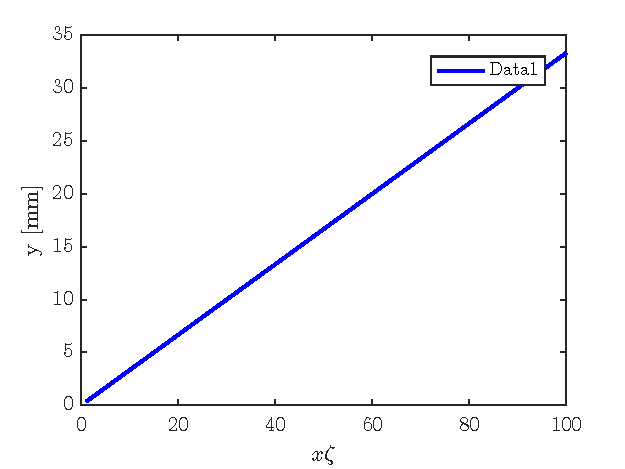
\includegraphics[width=.8\linewidth]{J100.pdf}
		%\caption{A new figure}
		\label{fig:}
	\end{figure} 
\end{frame}

\begin{frame}{Tikz Figure}
%\vspace*{2mm}
	\begin{figure}
		\setlength\figurewidth{0.9\textwidth}
		\setlength\figureheight{0.6\textwidth}
		\centering		
		% This file was created by matlab2tikz.
%
\begin{tikzpicture}

\begin{axis}[%
width=0.951\figurewidth,
height=\figureheight,
at={(0\figurewidth,0\figureheight)},
scale only axis,
xmin=0,
xmax=100,
xlabel style={font=\color{white!15!black}},
xlabel={$\zeta \cdot R_j P/A$ [\si{m^2}]},
ymin=-1,
ymax=9,
ylabel style={font=\color{white!15!black}},
ylabel={$\rho$ [\si{kg \per m}]},
axis background/.style={fill=white},
legend style={legend cell align=left, align=left, draw=white!15!black},
xlabel style={font=\footnotesize},ylabel style={font=\footnotesize},legend style={font=\sffamily\footnotesize,draw=TueText},ticklabel style={font=\sffamily\footnotesize}
]
\addplot [color=black, line width=1.0pt]
  table[row sep=crcr]{%
0	0\\
1	1\\
2	1.14869835499704\\
3	1.24573093961551\\
4	1.3195079107729\\
5	1.37972966146121\\
6	1.43096908110526\\
7	1.47577316159455\\
8	1.51571656651039\\
10	1.58489319246111\\
12	1.64375182951723\\
14	1.69521820307243\\
17	1.76234034783232\\
20	1.82056420302608\\
24	1.88817502258981\\
28	1.94729436123033\\
33	2.01234661708556\\
38	2.06993505408161\\
44	2.13152551327094\\
51	2.19540189742749\\
59	2.26032246962681\\
68	2.325422030439\\
78	2.39011567735218\\
90	2.45950948584937\\
100	2.51188643150958\\
};
\addlegendentry{Data1}

\addplot [color=red, dashed, line width=1.0pt]
  table[row sep=crcr]{%
0	0\\
1	0.824621125123528\\
2	1.16619037896906\\
3	1.42828568570857\\
4	1.64924225024707\\
5	1.84390889145858\\
6	2.01990098767241\\
7	2.18174242292714\\
8	2.33238075793813\\
9	2.4738633753706\\
10	2.60768096208106\\
11	2.73495886623547\\
12	2.85657137141715\\
13	2.9732137494637\\
14	3.0854497241083\\
16	3.29848450049413\\
18	3.49857113690717\\
20	3.68781778291715\\
22	3.86781592116274\\
24	4.03980197534483\\
26	4.20475920832573\\
28	4.36348484585429\\
30	4.51663591625449\\
33	4.7370877129308\\
36	4.9477267507412\\
39	5.14975727583349\\
42	5.34415568635495\\
45	5.53172667437573\\
48	5.71314274283428\\
52	5.94642749892741\\
56	6.1708994482166\\
60	6.38748776906853\\
64	6.59696900098825\\
68	6.8\\
73	7.04556598152341\\
78	7.28285658241325\\
83	7.51265598839719\\
88	7.73563184232549\\
94	7.99499843652268\\
100	8.24621125123532\\
};
\addlegendentry{Data2}

\addplot [color=blue, line width=1.0pt]
  table[row sep=crcr]{%
0	0\\
1	0.382573700617144\\
2	-0.344079280799377\\
3	-0.0197155586789393\\
4	-0.374374394899021\\
5	0.260837524580509\\
6	0.0749633946015678\\
7	0.325407878641897\\
8	-0.142419760286401\\
9	-0.15474786328771\\
10	-0.248330744741011\\
11	0.00442561130277852\\
12	0.242954412089972\\
13	0.160200962272569\\
14	0.134180633299053\\
15	-0.321252475419143\\
16	-0.0793787852135495\\
17	-0.254329383716339\\
18	0.372406635276803\\
19	0.0222094478043715\\
20	0.340123760557134\\
21	-0.38340646045171\\
22	-7.83426070682935e-05\\
23	-0.38155585001391\\
24	0.347857398902718\\
25	0.0173628855346806\\
26	0.376180603893403\\
27	-0.267206197688864\\
28	-0.0706455926815579\\
29	-0.329451965988582\\
30	0.15058126650419\\
31	0.149328414071206\\
32	0.253663452449402\\
33	-0.0132744069040456\\
34	-0.237538994620309\\
35	-0.16568328896382\\
36	-0.1258683218486\\
37	0.316989592772686\\
38	0.0838882578720188\\
39	0.247685032265096\\
40	-0.370279758044703\\
41	-0.0248425927079978\\
42	-0.335992363535169\\
43	0.384054706042505\\
44	0.000313309051918509\\
45	0.380352455989723\\
46	-0.351456709483571\\
47	-0.0151532768518479\\
48	-0.37782293512538\\
49	0.27343224072753\\
50	0.0664288055034348\\
51	0.333380970239531\\
52	-0.158660768589257\\
53	-0.143947001774052\\
54	-0.258948015550246\\
55	0.0221159231493999\\
56	0.232089049655229\\
57	0.171190389551768\\
58	0.117487312164485\\
59	-0.312623133611538\\
60	-0.0884882278393206\\
61	-0.240907820058112\\
62	0.367996300306658\\
63	0.0276129228620619\\
64	0.33168673409169\\
65	-0.384519137289402\\
66	-0.000704715249227661\\
67	-0.378963190175767\\
68	0.354875928026246\\
69	0.0130884680698244\\
70	0.379299169067167\\
71	-0.279512588363119\\
72	-0.0623163760760406\\
73	-0.337191196135748\\
74	0.166653939105046\\
75	0.13860797549863\\
76	0.264179938084027\\
77	-0.0309453126567689\\
78	-0.226609148445988\\
79	-0.176717781665275\\
80	-0.10904213734355\\
81	0.30815706447919\\
82	0.0931750348448759\\
83	0.234001187331984\\
84	-0.3655589013824\\
85	-0.0305182588907371\\
86	-0.327208634523998\\
87	0.38480057688308\\
88	0.00125225453592748\\
89	0.377387848810415\\
90	-0.358113891690422\\
91	-0.0111700803495154\\
92	-0.380607195445862\\
93	0.285444274300346\\
94	0.0583115619810286\\
95	0.340879023056885\\
96	-0.17455650948547\\
97	-0.133315643188723\\
98	-0.269354751026981\\
99	0.0397577363229402\\
100	0.22110387289159\\
};
\addlegendentry{Data3}

\end{axis}
\end{tikzpicture}%
		%\caption{Kas is dken ok}
		\label{kalsd}
	\end{figure}
\end{frame}

\begin{frame}{Laminar flow: single jet burner}
\begin{figure}[H] 
		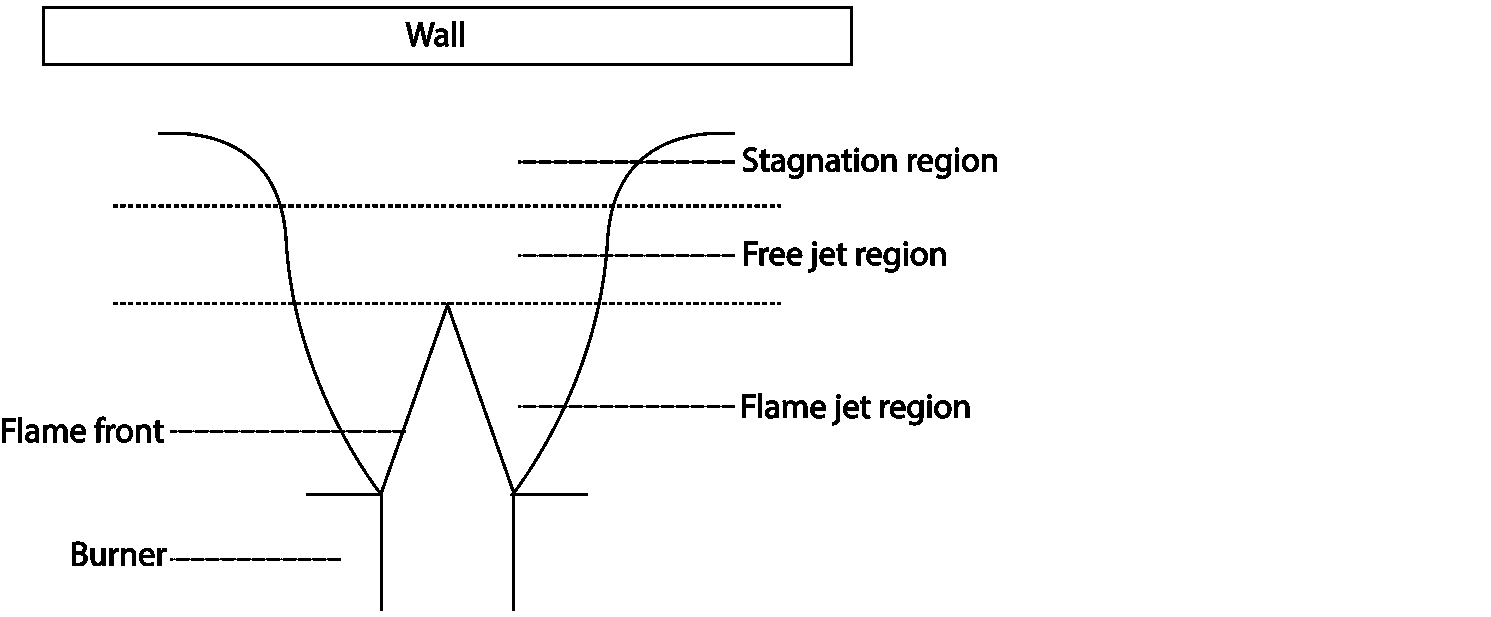
\includegraphics[width=\linewidth]{Laminar2.png} 
	\end{figure}
\end{frame}

\begin{frame}{Laminar flow: single jet burner}
	\begin{figure}[H]
		\centering 
		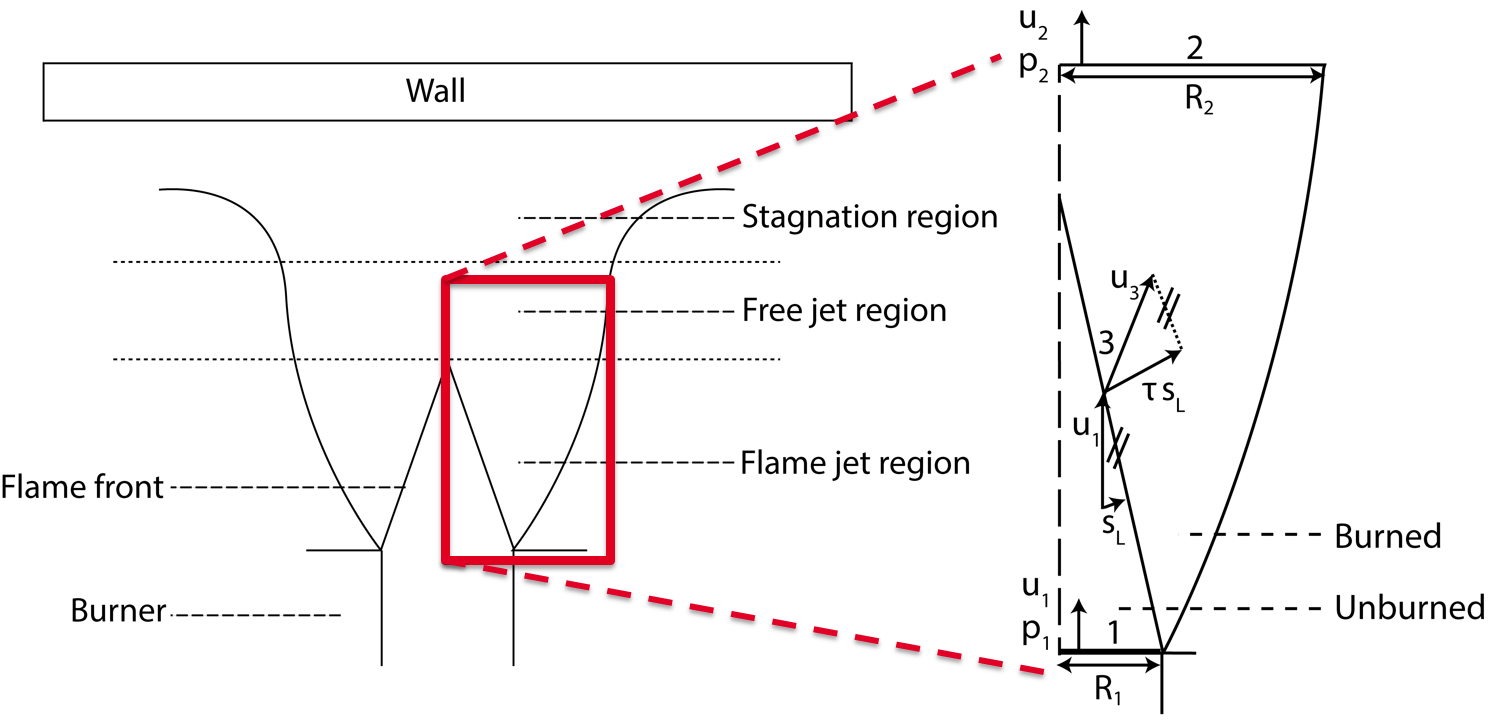
\includegraphics[width=\linewidth]{Laminar.png}
	\end{figure}
\end{frame}



\section{Theory}
\begin{frame}{Stagnation point}
\newcommand{\Rey}{\operatorname{\mathit{\mathcal{R}\kern-.14em e}}}

\newcommand{\Web}{\operatorname{\mathit{\mathcal{W}\kern-.14em e}}}

\newcommand{\Pec}{\operatorname{\mathit{\mathcal{P}\kern-.14em e}}}

\newcommand{\Capi}{\operatorname{\mathit{\mathcal{C}\kern-.14em a}}}
sdfsdfsdcxvxcv
$
	\Capi
	\Web
	\Rey
	\Pec
	$
	\[
		q(r) = q_s \exp \left(-0.45\frac{r}{R_2} - 1 \right)
	\]
	\[		h = 0.763 \sqrt{\beta^{1.5} \rho_u \mu} \Rey^{0.6} c_p \Capi_i x \Web^{5.2} \delta_{ij}
	\]
 \end{frame}
\section{Movies}
\begin{frame}{Movie time}
\begin{center}%
    \includemovie{Marangoni.mp4}%
\newline
The Marangoni Effect
\\
{\scriptsize \url{https://www.youtube.com/watch?v=0h16Tyn2138}}
\end{center}%
\end{frame}

\begin{frame}[standout]{TO DO}
	\begin{itemize}
		\item structuur \\
		\item Matlab script\\
	\end{itemize}
\end{frame}

\begin{frame}{Conclusions/Summary}
	\begin{itemize}
		\item Cost reduction by changing burner configuration
		\item Burner to pile
	\end{itemize}
\end{frame}

{\setbeamercolor{background canvas}{bg=TueRed}
\begin{frame}{}  
	\begin{center}
	\color{white}{\Large{\textbf{Questions?}}}
	\end{center}
\end{frame}
}

\begin{frame}
	\vspace*{3em}
	\begin{columns}[onlytextwidth,c]
		\column{0.1\textwidth}
    	\column{0.35\textwidth}
    	\textbf{Twan Bouts}
    	
    	\column{0.55\textwidth}
    	{\scriptsize
    	Eindhoven University of Technology\\
    	Department of Mechanical Engineering\\
    	Microsystems\\
		\vspace*{1em}
    	\href{mailto:t.m.j.bouts@student.tue.nl}{t.m.j.bouts@student.tue.nl}\\
    	%\href{https://www.tue.nl/en/research/research-groups/microsystems/}{https://www.tue.nl/en/research/research-groups/microsystems/}
    	}
    \end{columns}
    \vspace*{1em}
    %{\scriptsize\href{https://www.tue.nl/en/research/research-groups/microsystems/}{https://www.tue.nl/en/research/research-groups/microsystems/}}
\end{frame}
%%%%%%%%%%%%%%%%%%%%%%%%%%%%%%%%%%%%%%%%%%%%%%%%%%%%%%%%%%%%%%%%%%%%%%%%%%%%%%%%%
%%%%%						END OF REGULAR PRESENTATION						%%%%%
%%%%%%%%%%%%%%%%%%%%%%%%%%%%%%%%%%%%%%%%%%%%%%%%%%%%%%%%%%%%%%%%%%%%%%%%%%%%%%%%%

\appendix
\begin{frame}[fragile]{Backup slides}
  Sometimes, it is useful to add slides at the end of your presentation to
  refer to during audience questions.

  The best way to do this is to include the \verb|appendixnumberbeamer|
  package in your preamble and call \verb|\appendix| before your backup slides.

  will automatically turn off slide numbering and progress bars for
  slides in the appendix.
\end{frame}

\begin{frame}{Blockies}
  Just some random text to prove that these blocks can be incorporated within a slide
   \begin{block}{Formulae}
	$ F = m \cdot a = m \dfrac{\partial^2 x}{\partial t^2 }$
   \end{block}
  If you are keen on writing some more, you could do it here.
   \begin{definition}
   		Newton says, force is mass times acceleration
   \end{definition}
    It's even possible to write under the blocks
\end{frame}

\begin{frame}{Tables}

\begin{center}
\begin{table}
\centering\caption{Properties of different fuels for current situation (Factory specs) and at the highest $T_{flame}$ (Optimal)}
\footnotesize{
\begin{tabular}{ l  l  l  l  l l} 
Fuel & Setting & $s_L [\frac{cm}{s}]$ & $T_{flame} [K]$ & $\rho _u [\frac{kg}{m^3}]$ & $\rho _b [\frac{kg}{m^3}]$ \vspace{1mm} \\ \hline 
\ce{CH4 - O2} & Optimal  & 306 & 3055.43 & 1.0961 & 0.0830 \\
& Factory & 306 & 3051.62 & 1.1091 & 0.0859 \vspace{1mm} \\ 
 \ce{C3H8 - O2} & Optimal  & 353 & 3100.85 & 1.4238 & 0.0858 \\
& Factory & 353 & 3064.47 & 1.4427 & 0.0796 \\  
\end{tabular}}
\end{table}
\end{center}
\end{frame}

\begin{frame}[noframenumbering,plain,allowframebreaks]{References}
\renewcommand*{\bibfont}{\scriptsize}
    \printbibliography[heading=none]
\end{frame}

%\endgroup 	
\end{document}
